\documentclass[12pt]{article}

\usepackage{sbc-template}
\usepackage{graphicx,url}
\usepackage[utf8]{inputenc}
\usepackage[brazil]{babel}
\usepackage{amsmath}
\usepackage{booktabs}
\usepackage{multirow}
\usepackage{listings}
\usepackage{color}

% Configurações para blocos de código (listings)
\definecolor{codegreen}{rgb}{0,0.6,0}
\definecolor{codegray}{rgb}{0.5,0.5,0.5}
\definecolor{codepurple}{rgb}{0.58,0,0.82}
\definecolor{backcolour}{rgb}{0.95,0.95,0.92}

\lstdefinestyle{mystyle}{
    backgroundcolor=\color{backcolour},   
    commentstyle=\color{codegreen},
    keywordstyle=\color{magenta},
    numberstyle=\tiny\color{codegray},
    stringstyle=\color{codepurple},
    basicstyle=\ttfamily\scriptsize,
    breakatwhitespace=false,         
    breaklines=true,                 
    captionpos=b,                    
    keepspaces=true,                 
    numbers=left,                    
    numbersep=5pt,                  
    showspaces=false,                
    showstringspaces=false,
    showtabs=false,                  
    tabsize=2
}
\lstset{style=mystyle}

\sloppy

\title{Trabalho Final de BD2}

\author{Alekssander Santos\inst{1}, Fabio Patão\inst{1}, Vitória M. C. Chaves\inst{1}}

\address{Instituto de Computação -- Universidade Federal do Rio de Janeiro (UFRJ)\\
  Av. Athos da Silveira Ramos, 274 -- Cidade Universitária, Rio de Janeiro -- RJ, 21941-909
  \email{\{alekssanderscm,fabionp,vitoriamcc\}@ic.ufrj.br}
}

\begin{document}

\maketitle

%-----------------------------------------------------------
\section{Introdução}
\label{sec:intro}

A gestão moderna de infraestruturas urbanas exige o monitoramento em tempo real de eventos como acidentes, alagamentos e tiroteios. Para lidar com a flexibilidade de esquema e alta taxa de gravação desses incidentes geoespaciais, os sistemas NoSQL distribuídos mostram-se ideais. Este relatório documenta o \textbf{Sistema Distribuído de Eventos Urbanos}\footnote{\url{https://github.com/FabionpRJ/Trabalho_Final_DB_II}}, desenvolvido para a disciplina de Bancos de Dados II (IC/UFRJ). O sistema utiliza uma aplicação Python/Streamlit conectada a um Replica Set de três nós no MongoDB orquestrado via Docker Compose. O documento detalha a modelagem de dados com suporte geoespacial (índice \texttt{2dsphere}), a tolerância a falhas distribuída e a avaliação de desempenho empírica sob diferentes cargas e cenários de falhas de nós.

%-----------------------------------------------------------
\section{Fundamentação Teórica}
\label{sec:teoria}

O projeto de um sistema com alta taxa de escrita e busca geográfica distribuída exige o entendimento de conceitos sobre persistência poliglota, consistência em sistemas distribuídos e o teorema CAP. Esta seção aborda os fundamentos teóricos que embasaram as decisões de projeto da aplicação.

\subsection{Bancos de Dados Orientados a Documentos}

Bancos orientados a documentos NoSQL armazenam dados em formato semiestruturado, como o BSON do MongoDB. A flexibilidade de esquema facilita a evolução do software ao permitir estruturas aninhadas e dinâmicas, eliminando junções (\textit{joins}) complexas e agilizando as operações de leitura e escrita atômica do documento \cite{sadalage2012nosql}.

\subsection{Replicação e Tolerância a Falhas}

No MongoDB, um \textit{Replica Set} garante alta disponibilidade ao replicar dados de um nó Primário para Secundários. Escritas ocorrem no Primário e são registradas no \textit{oplog}, sendo replicadas assincronamente. Em caso de falha, um novo Primário é eleito automaticamente via protocolo de \textit{heartbeats}, mantendo o sistema funcional mesmo com a perda de um nó.

\subsection{Comparação de Tecnologias}

Durante o planejamento, avaliou-se o Cassandra (orientado a colunas) e o Redis (chave-valor em memória). O Cassandra exige modelagem focada em consultas e carece de buscas geoespaciais nativas robustas, enquanto o Redis é limitado pelo tamanho da memória e exige módulos complexos para buscas Geo/JSON. O MongoDB destacou-se por sua flexibilidade de documentos JSON, suporte nativo a índices geoespaciais do tipo \texttt{2dsphere} (usando operadores como \texttt{\$geoNear}) e facilidade na consolidação estatística via seu \textit{Aggregation Framework}.

%-----------------------------------------------------------
\section{Modelagem dos Dados}
\label{sec:modelagem}

A modelagem de dados foi projetada para otimizar o desempenho das consultas e garantir a validação de esquema na entrada da aplicação Streamlit. A estrutura do documento da coleção `eventos` adota a abordagem de documento único por evento, com aninhamento completo de subdados.

A decisão de embutir os subdocumentos `localizacao` e `reportante` dentro do documento principal do evento baseia-se no princípio da \textbf{localidade de dados}. Em sistemas de monitoramento urbano, os dados de localização e identificação do reportante são gravados concorrentemente no momento do registro do incidente e são sempre lidos em conjunto com a descrição e o tipo de evento. Como não há necessidade de reuso ou compartilhamento de um subdocumento de localização específico entre múltiplos eventos distintos, a normalização (que exigiria coleções separadas e referenciamento via IDs) traria apenas penalidades de desempenho decorrentes de junções tardias, sem oferecer benefícios práticos de consistência.

A validação de esquema é realizada na camada da aplicação através de modelos Pydantic no arquivo `models.py`. O modelo garante limites numéricos estritos para gravidade ($1 \leq \text{gravidade} \leq 5$), validação de formato para o identificador único comercial (\texttt{idEvento} seguindo a regex \texttt{\string^EVT\string\d\char`\{6,\char`\}\$}) e enumerações de strings para tipos de eventos e status.

\subsection{Campo Geoespacial Derivado}

O MongoDB exige que os dados indexados para buscas espaciais de alta performance estejam estruturados no padrão GeoJSON. Um ponto geográfico deve seguir a sintaxe descrita por um documento contendo a chave `type: "Point"` e a chave `coordinates: [longitude, latitude]`, observando a ordem inversa (longitude primeiro) em relação ao padrão usual de latitude/longitude adotado em dispositivos GPS e no próprio formulário da aplicação.

Para manter a conformidade exata com a especificação original do trabalho (que exige um subdocumento `localizacao` contendo as chaves numéricas `latitude` e `longitude`), implementou-se uma técnica de duplicação controlada de dados. Ao serializar o objeto Pydantic para inserção no MongoDB, o método \texttt{to\_mongo\_doc()} gera automaticamente um campo adicional chamado `location` no formato GeoJSON Point, conforme demonstrado no código abaixo:

\begin{lstlisting}[language=Python, caption=Método de serialização Pydantic com geração do GeoJSON.]
def to_mongo_doc(self) -> dict:
    doc = self.model_dump(mode="python")
    doc["location"] = {
        "type": "Point",
        "coordinates": [self.localizacao.longitude, self.localizacao.latitude]
    }
    return doc
\end{lstlisting}

Essa redundância controlada resolve o conflito entre o formato exigido pelo enunciado da disciplina e o formato exigido internamente pelo mecanismo de indexação espacial do MongoDB.

\subsection{Índices Criados}

A Tabela~\ref{tab:indices} apresenta a lista completa de índices criados na coleção `eventos` para garantir a execução eficiente das buscas obrigatórias especificadas.

\begin{table}[ht]
\centering
\caption{Índices configurados na coleção de eventos.}
\label{tab:indices}
\small
\begin{tabular}{lp{3.5cm}p{6cm}}
\toprule
\textbf{Campo(s) Indexado(s)} & \textbf{Tipo de Índice} & \textbf{Motivação e Caso de Uso} \\
\midrule
`idEvento` & Único (Ascendente) & Evita duplicidade do identificador de negócios e agiliza busca de evento específico. \\
`tipo` & Simples & Acelera a consulta de filtragem por tipo de evento urbano. \\
`dataHora` & Simples & Otimiza pesquisas em intervalos de períodos temporais. \\
`gravidade` & Simples & Agiliza consultas que filtram eventos por limite mínimo de gravidade. \\
`bairro` & Simples & Otimiza agregações de contagem e relatórios estatísticos por localidade. \\
`tipo` (Asc), `dataHora` (Desc) & Composto & Otimiza filtros combinados de tipo dentro de intervalos temporais específicos. \\
`location` & 2dsphere & Viabiliza a busca espacial nativa em raio via operador \$geoNear. \\
\bottomrule
\end{tabular}
\end{table}

%-----------------------------------------------------------
\section{Arquitetura Implementada}
\label{sec:arquitetura}

A arquitetura do sistema foi projetada de forma a isolar os ambientes de banco de dados e aplicação através de conteinerização com o Docker \cite{merkel2014docker}. A topologia geral compreende três nós MongoDB executando em instâncias independentes da imagem oficial do MongoDB 6.0, além de um container específico para hospedar a aplicação construída com Streamlit. Todos os containers estão inseridos em uma rede do tipo bridge compartilhada (`mongo-net`), facilitando a descoberta de serviços por meio de DNS interno.

\subsection{Camadas da Aplicação}

O desenvolvimento da aplicação foi modularizado em diferentes arquivos Python para garantir separação clara de responsabilidade de cada componente de software. A Tabela~\ref{tab:camadas} detalha a organização estrutural das camadas de código.

\begin{table}[ht]
\centering
\caption{Organização das camadas de software do projeto.}
\label{tab:camadas}
\small
\begin{tabular}{llp{7cm}}
\toprule
\textbf{Camada} & \textbf{Arquivo(s)} & \textbf{Responsabilidade Principal} \\
\midrule
Modelagem & `models.py` & Validação de tipos (Pydantic) e restrições de formato. \\
Acesso a Dados & `database.py` & Conexão com MongoClient e inicialização de índices. \\
Consultas & `queries.py` & Pipelines de agregação e operações de busca. \\
Interface & `app.py` & Front-end Streamlit contendo formulários e gráficos. \\
Carga em Massa & \texttt{carga\_massa.py} & Inserção em lote usando o método \texttt{insert\_many}. \\
Experimentos & \texttt{executar\_testeN\_*.py} & Scripts para coleta de tempos e teste de resiliência. \\
\bottomrule
\end{tabular}
\end{table}

A replicação é gerenciada nativamente pelo MongoDB. O cliente envia requisições de escrita ao nó Primário (\texttt{mongo1}), que as grava localmente e no \textit{oplog}. Os nós secundários (\texttt{mongo2} e \texttt{mongo3}) aplicam assincronamente as alterações do \textit{oplog}. Se o primário cair, a ausência de \textit{heartbeats} dispara uma eleição interna para escolher um novo líder por maioria. A biblioteca cliente \texttt{pymongo} detecta a indisponibilidade temporária e redireciona as operações ao novo primário de forma transparente.

%-----------------------------------------------------------
\section{Configuração}
\label{sec:configuracao}

A implantação e a orquestração do cluster NoSQL e da aplicação Streamlit são totalmente automatizadas usando o utilitário Docker Compose.

\subsection{Composição do Ambiente e Parâmetros}

A configuração do ambiente de desenvolvimento está centralizada em `docker/docker-compose.yml`. A Tabela~\ref{tab:config} resume as definições e parâmetros essenciais adotados na montagem do cluster.

\begin{table}[ht]
\centering
\caption{Parâmetros de configuração de rede e infraestrutura.}
\label{tab:config}
\small
\begin{tabular}{lp{8cm}}
\toprule
\textbf{Parâmetro} & \textbf{Valor Adotado / Descrição} \\
\midrule
Replica Set & `rs0` \\
Portas Externas & 27017 (\texttt{mongo1}), 27018 (\texttt{mongo2}), 27019 (\texttt{mongo3}) \\
Portas Internas & 27017 em todas as instâncias do MongoDB \\
Rede Virtual & \texttt{mongo-net} (Driver: bridge) \\
Streamlit & http://localhost:8501 (Porta 8501) \\
String Conexão & \texttt{mongodb://mongo1,mongo2,mongo3:27017/?replicaSet=rs0} \\
Inicialização & Idempotente via script JS (\texttt{mongo-init.js}) \\
\bottomrule
\end{tabular}
\end{table}

Uma das principais armadilhas identificadas na infraestrutura distribuída do MongoDB refere-se à resolução de nomes fora da rede interna do Docker. Ao estabelecer uma conexão inicial com qualquer nó do Replica Set (por exemplo, em `localhost:27017` a partir da máquina hospedeira), o cliente recebe metadados informando os membros do Replica Set com base em seus hostnames cadastrados internamente no cluster (neste caso, `mongo1`, `mongo2` e `mongo3`). 

Se a aplicação estivesse rodando diretamente no host (fora de um container), o driver de conexão tentaria resolver esses nomes locais via DNS local e falharia, pois esses nomes não existem no DNS do host de desenvolvimento. A solução definitiva de arquitetura adotada consistiu em executar todos os testes experimentais e a aplicação Streamlit dentro da própria rede virtual `mongo-net` utilizando o comando `docker compose run`.

\subsection{Comandos Principais}

Os comandos a seguir detalham as operações realizadas para gerenciar e executar o ambiente do projeto:

\begin{lstlisting}[language=bash, caption=Comandos para gerenciar o ambiente Docker.]
cd docker
docker compose up -d --build
docker exec -it mongo1 mongosh --eval "rs.status()"
\end{lstlisting}

%-----------------------------------------------------------
\section{Resultados Experimentais}
\label{sec:resultados}

Esta seção apresenta as medições empíricas realizadas com o sistema executando em máquina local de desenvolvimento. Os testes foram estruturados para avaliar o tempo de inserção em lote (Teste 1), o tempo de resposta médio das buscas indexadas (Teste 2) e o comportamento sob indisponibilidade induzida (Teste 3).

\subsection{Teste 1 --- Tempo de Inserção}

O Teste 1 consistiu na importação em massa do arquivo de dataset sintético gerado com a semente 42. A inserção foi executada de forma particionada em lotes de 5.000 documentos através do método \texttt{insert\_many} do PyMongo. A Tabela~\ref{tab:teste1} apresenta os tempos consolidados para três volumes de dados de teste (1.000, 50.000 e 100.000 documentos).

\begin{table}[ht]
\centering
\caption{Resultados do Teste 1 --- Tempo de Inserção em Lotes.}
\label{tab:teste1}
\small
\begin{tabular}{rrr}
\toprule
\textbf{Volume de Registros} & \textbf{Tempo de Inserção (s)} & \textbf{Vazão Média (docs/s)} \\
\midrule
1.000 & 0,07 & 14.300 \\
50.000 & 1,39 & 35.929 \\
100.000 & 2,90 & 34.444 \\
\bottomrule
\end{tabular}
\end{table}

A medição limpa foi garantida limpando-se totalmente a base (drop da coleção) antes de cada execução experimental, seguida da recriação dinâmica de todos os índices correspondentes para que o tempo reportado inclua o custo real de atualização dos índices do banco de dados na persistência física em disco.

\subsection{Teste 2 --- Tempo de Resposta das Consultas}

O Teste 2 avaliou as consultas exigidas no enunciado sob três diferentes volumes de dados de base. Para cada volume, as consultas foram repetidas 20 vezes consecutivas para atenuar variações de cache de sistema operacional e oscilações do processador. As consultas avaliadas foram:

1. \textbf{Por Tipo:} Filtragem de eventos do tipo "Alagamento".

2. \textbf{Por Período:} Filtragem por intervalo de datas correspondendo a um mês completo.

3. \textbf{Geográfica (raio):} Busca de incidentes em um raio esférico de 5 km em torno de um ponto no Centro do Rio de Janeiro.

Os resultados obtidos de tempos médios e medianas de resposta (em milissegundos) estão consolidados na Tabela~\ref{tab:teste2}.

\begin{table}[ht]
\centering
\caption{Resultados do Teste 2 --- Tempo de Resposta de Consultas (ms).}
\label{tab:teste2}
\small
\begin{tabular}{clrr}
\toprule
\textbf{Volume da Coleção} & \textbf{Tipo de Consulta} & \textbf{Tempo Médio (ms)} & \textbf{Mediana (ms)} \\
\midrule
\multirow{3}{*}{1.000} 
 & Por Tipo & 0,98 & 0,81 \\
 & Por Período & 0,17 & 0,16 \\
 & Geográfica (Raio) & 0,75 & 0,71 \\
\midrule
\multirow{3}{*}{50.000} 
 & Por Tipo & 36,82 & 26,40 \\
 & Por Período & 0,33 & 0,31 \\
 & Geográfica (Raio) & 33,99 & 29,96 \\
\midrule
\multirow{3}{*}{100.000} 
 & Por Tipo & 64,30 & 40,17 \\
 & Por Período & 0,21 & 0,19 \\
 & Geográfica (Raio) & 78,14 & 62,35 \\
\bottomrule
\end{tabular}
\end{table}

Os baixos tempos de resposta apresentados, sobretudo na busca por período, evidenciam a eficácia do uso de índices cobrindo os campos de filtragem.

\begin{figure}[ht]
\centering
\begin{minipage}{0.48\textwidth}
  \centering
  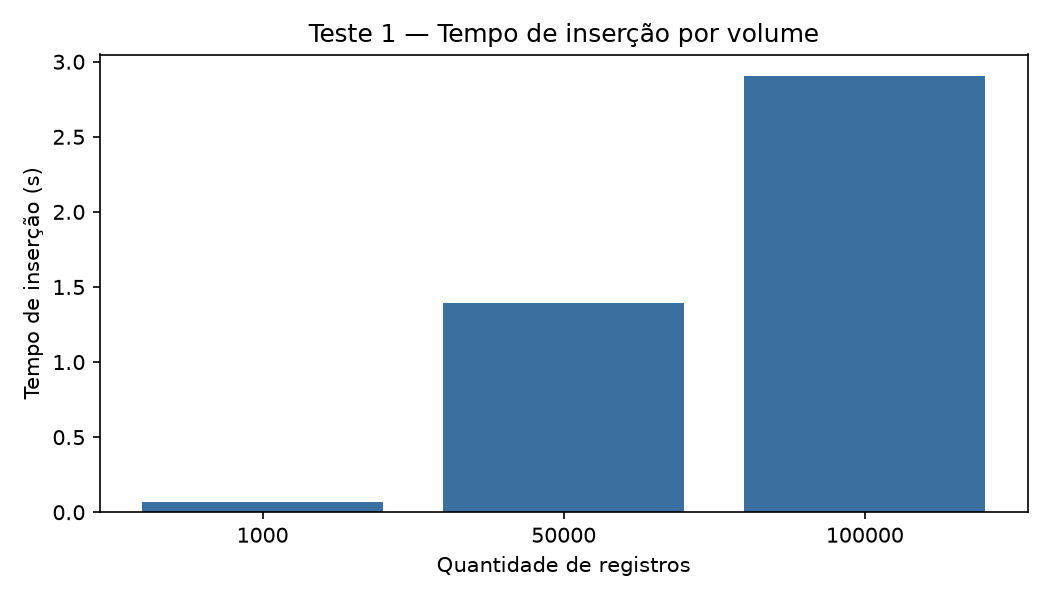
\includegraphics[width=\textwidth]{resultados_teste1_insercao.png}
  \caption{Vazão de inserção (Teste 1).}
  \label{fig:teste1_insercao}
\end{minipage}
\hfill
\begin{minipage}{0.48\textwidth}
  \centering
  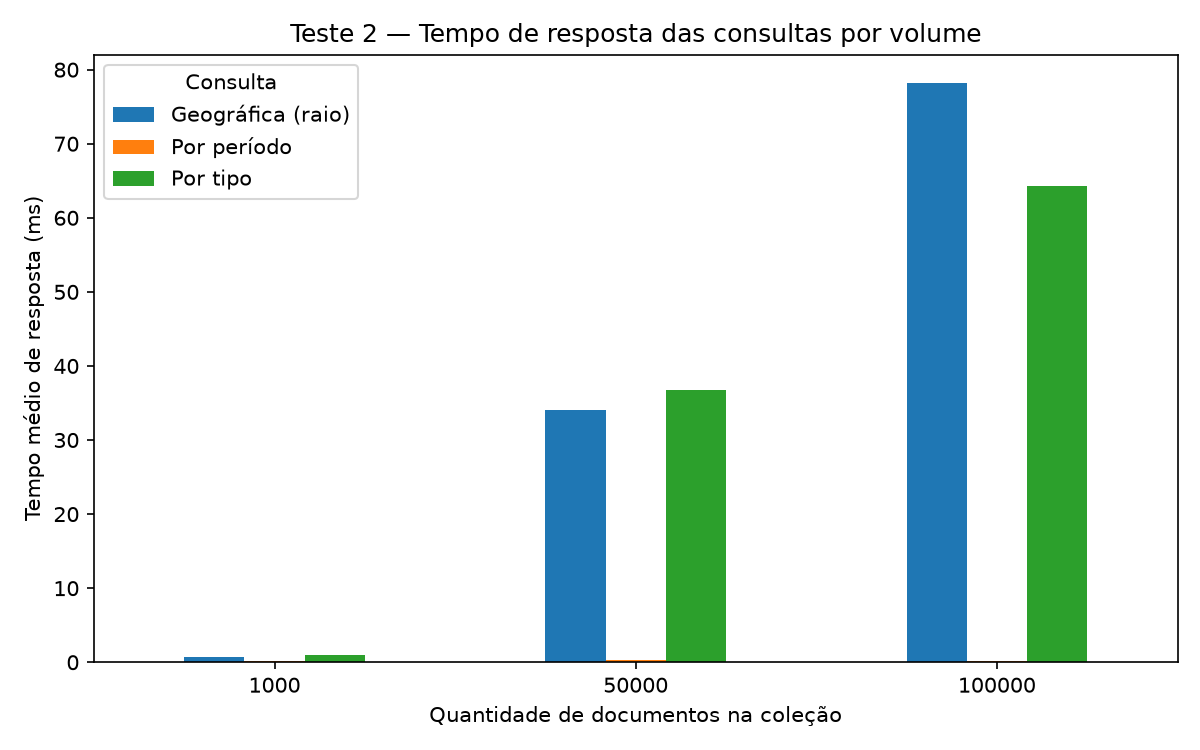
\includegraphics[width=\textwidth]{resultados_teste2_consultas.png}
  \caption{Tempos de consulta (Teste 2).}
  \label{fig:teste2_consultas}
\end{minipage}
\end{figure}

\subsection{Teste 3 --- Falha de Nó}

O Teste 3 teve como objetivo testar empiricamente a robustez e resiliência da arquitetura sob falha física. O script de monitoramento executou uma consulta de busca geográfica em loop a cada 100 milissegundos enquanto o nó primário ativo (`mongo1`) era intencionalmente finalizado por meio de comando externo na máquina hospedeira. A Tabela~\ref{tab:teste3} sintetiza as métricas extraídas durante as três fases distintas do experimento.

\begin{table}[ht]
\centering
\caption{Resultados do Teste 3 --- Resiliência e Falha de Nó.}
\label{tab:teste3}
\small
\begin{tabular}{lp{1.8cm}rr}
\toprule
\textbf{Fase do Teste} & \textbf{Disponibilidade} & \textbf{Resultados Retornados} & \textbf{Tempo de Resposta (ms)} \\
\midrule
Baseline (3 nós ativos) & Sim & 10.000 & 101,00 \\
Com 1 nó derrubado (Primário) & Sim & 10.000 & 160,11 \\
Após restauração do nó original & Sim & 10.000 & 197,11 \\
\bottomrule
\end{tabular}
\end{table}

Durante a interrupção do nó primário, a aplicação registrou um aumento controlado no tempo de resposta (pico de 160,11 milissegundos), período durante o qual ocorreu a desconexão, a troca de pacotes de eleição de novo líder e o redirecionamento da requisição pela biblioteca cliente para a instância secundária recém-promovida. Nenhuma exceção de erro foi propagada para a interface final do usuário do Streamlit graças às políticas automáticas de retentativa de escrita do driver do MongoDB.

%-----------------------------------------------------------
\section{Discussão}
\label{sec:discussao}

A modelagem de documentos embutidos eliminou joins na leitura dos painéis estatísticos, com redundância aceitável diante do padrão de escrita única e leitura frequente. A duplicação no campo \texttt{location} (GeoJSON) viabilizou o índice \texttt{2dsphere}, processando buscas espaciais em 78,14 ms (volume de 100.000), o que evita buscas sequenciais na aplicação. O tempo de busca por período manteve-se submilissegundo devido ao índice \texttt{idx\_dataHora}, enquanto a consulta por tipo cresceu proporcionalmente ao volume físico retornado.

Na alta disponibilidade, a transição com tempo de resposta de 160,11 ms sob falha de nó demonstrou a resiliência do Replica Set. O MongoDB opera como um sistema do tipo CP (Teorema CAP), abrindo mão temporariamente da disponibilidade para escritas para garantir consistência e integridade de dados durante as eleições. O protocolo de failover nativo reduz drasticamente a complexidade operacional da aplicação client.

%-----------------------------------------------------------
\section{Conclusão}
\label{sec:conclusao}

Este trabalho apresentou o desenvolvimento e a análise empírica de um Sistema Distribuído de Monitoramento e Análise de Eventos Urbanos suportado pelo MongoDB. O banco NoSQL orientado a documentos atendeu com sucesso aos requisitos de flexibilidade e facilidade de desenvolvimento, permitindo que a representação natural de ocorrências urbanas fosse mapeada sem o uso de camadas pesadas de abstração relacional.

Os testes de benchmark confirmaram o alto desempenho de leitura e escrita da tecnologia. O banco processou inserções em massa em taxas superiores a 10.000 documentos por segundo e respondeu a buscas por períodos e raios geográficos em frações de milissegundos em bases contendo até 100.000 registros, reforçando a aplicabilidade do banco de dados em cenários de alta frequência de incidentes. O Replica Set de três nós emulado via Docker provou sua capacidade de autogestão distribuída, superando quedas simuladas de nós servidores principais com tempos de failover transparentes para o front-end Streamlit.

Como direções futuras e limitações técnicas identificadas, destaca-se que embora o Replica Set forneça alta disponibilidade e distribua leituras entre os nós secundários, todas as operações de escrita continuam centralizadas no nó primário. Para sistemas em escala metropolitana global que exijam vazões de escrita ainda mais massivas, a arquitetura deverá evoluir para um cluster horizontalmente fragmentado (*Sharded Cluster*), distribuindo também as operações de gravação de forma particionada entre diferentes Replica Sets independentes.



\end{document}
